\documentclass[aspectratio=169,10pt]{beamer}

\usetheme{Madrid}
\usecolortheme{seahorse}
\setbeamertemplate{footline}[frame number]

\usepackage{amsmath,amssymb,amsfonts,xcolor}
\usepackage{graphicx}
\usepackage{listings}
\usepackage{xcolor}
\usepackage{tikz}
\usetikzlibrary{arrows, positioning, shapes, matrix}

\graphicspath{{figures/}}

% Custom colors
\definecolor{darkblue}{rgb}{0,0,0.5}
\definecolor{darkgreen}{rgb}{0,0.5,0}
\definecolor{darkred}{rgb}{0.5,0,0}

% Code listing style
\lstset{
    basicstyle=\ttfamily\scriptsize,
    keywordstyle=\color{blue}\bfseries,
    commentstyle=\color{darkgreen}\itshape,
    stringstyle=\color{darkred},
    numberstyle=\tiny\color{gray},
    numbers=left,
    frame=single,
    breaklines=true,
    language=Python,
    showstringspaces=false,
}

\title{Chapter 9: Applications of Fixed Point Theorems}
\subtitle{Applications to Integral and Volterra Equations, Surjectivity Theorems}
\author{Based on Pathak: Introduction to Nonlinear Analysis and Fixed Point Theory}
\date{Pages 738--757}

\begin{document}

%==============================================================================
% TITLE SLIDE
%==============================================================================
\begin{frame}
\titlepage
\end{frame}

%==============================================================================
% TABLE OF CONTENTS
%==============================================================================
\begin{frame}[allowframebreaks]{Outline}
\begin{itemize}
    \item \textbf{Section 9.5:} Application to Nonlinear Integral Equations
    \begin{itemize}
        \item The integral equation framework
        \item Darbo's fixed point theorem application
        \item Special cases of classical integral equations
    \end{itemize}
    \vspace{0.3cm}
    \item \textbf{Section 9.6:} Application to Volterra Integrodifferential Equations
    \begin{itemize}
        \item Volterra equations of the second kind
        \item Existence and uniqueness theorems
        \item Lipschitz continuity and regularity
    \end{itemize}
    \vspace{0.3cm}
    \item \textbf{Section 9.7:} Application to Surjectivity Theorems
    \begin{itemize}
        \item Generalized directional contractors
        \item Class (S) contractors
        \item Existence of solutions to operator equations
    \end{itemize}
\end{itemize}
\end{frame}

%==============================================================================
% SECTION 9.5: NONLINEAR INTEGRAL EQUATIONS
%==============================================================================
\section{Application to Nonlinear Integral Equations}

\begin{frame}{Section 9.5: Nonlinear Integral Equations}{Problem Framework}
We consider the integral equation of the form
\[
x(t) = u(t, x(t)) + \int_0^t p(t, s, x(s)) ds, \quad t \in [0, a]
\]
where
\begin{itemize}
    \item $u : [0, a] \times \mathbb{R} \to \mathbb{R}$ is continuous
    \item $p : [0, a] \times [0, a] \times \mathbb{R} \to \mathbb{R}$ is continuous
    \item $g : [0, a] \times [0, a] \to \mathbb{R}^+$ is a continuous bound
\end{itemize}

\medskip

This is a classical nonlinear Volterra integral equation that arises in many applied problems.
\end{frame}

\begin{frame}{Fixed Point Formulation}{Mapping on $C[0,a]$}
Define the operator $T : C[0, a] \to C[0, a]$ by
\[
(Tx)(t) = u(t, x(t)) + \int_0^t p(t, s, x(s)) ds
\]

Finding a solution to the integral equation is equivalent to finding a fixed point of $T$.

\medskip

\textbf{Key Step:} Show that $T$ satisfies the \alert{Darbo condition}:
\[
\mu(TX) \leq q \mu(X) \quad \text{for some } q < 1
\]

where $\mu$ denotes the Kuratowski measure of noncompactness.
\end{frame}

\begin{frame}{Assumptions for Existence}{Conditions A1--A4}
\begin{itemize}
    \item[\textbf{A1:}] There exist constants $k, k', a \beta$ and a nondecreasing function $\phi : [0, \infty) \to [0, \infty)$ with $\phi(0) = 0$ such that
    \[
    |u(t, x) - u(t, y)| \leq k|x - y|, \quad |p(t, s, x) - p(t, s, y)| \leq a\phi(|x - y|)
    \]
    for all $t, s \in [0, a]$ and $x, y \in \mathbb{R}$.

    \vspace{0.2cm}
    \item[\textbf{A2:}] $|u(t, 0)| \leq m$ and $|p(t, s, 0)| \leq \psi(t, s)$ for some $m \geq 0$ and measurable function $\psi$.

    \vspace{0.2cm}
    \item[\textbf{A3:}] $\gamma = k + ka\beta < 1$.

    \vspace{0.2cm}
    \item[\textbf{A4:}] $\eta = ka\ell + m$ where $\ell = \max_{t,s} |g(t,s)|$.
\end{itemize}
\end{frame}

\begin{frame}{Contraction Property of $T$}{Darbo Condition Analysis}
From assumptions A1--A4, we can show that the operator $T$ maps the ball
\[
B_r = \{x \in C[0, a] : \|x\| \leq r\} \quad \text{into itself}
\]
where $r_1 \leq r \leq r_2$ with
\[
r_1 = \frac{(1 - 2y\eta) - \sqrt{1 - 4y\eta}}{2y^2}, \quad r_2 = \frac{(1 - 2y\eta) + \sqrt{1 - 4y\eta}}{2y^2}
\]

\medskip

Furthermore, the operator $T$ satisfies the Darbo condition with respect to the measure $\omega_0$:
\[
\omega_0(TX) \leq 2k\omega_0(X), \quad \omega_0(GX) \leq 2k\omega_0(X)
\]

Hence $T$ is a contraction with respect to $\omega_0$ and has at least one fixed point.
\end{frame}

\begin{frame}[allowframebreaks]{Special Cases of Integral Equations}{}
The equation $x(t) = u(t, x(t)) + \int_0^t p(t, s, x(s)) ds$ encompasses many classical forms:

\medskip
\textbf{Case 1:} If $g(t, y, x) = 1$, then
\[
x(t) = u(t, x(t)) + \int_0^t p(t, s, x(s)) ds \quad \text{[Ref. 380]}
\]

\medskip
\textbf{Case 2:} For $u(t, x) = 0$, we get the nonlinear functional-integral equation
\[
x(t) = f\left(t, \int_0^t p(t, s, x(s)) ds\right) \cdot g\left(t, \int_0^a q(t, s, x(s)) ds\right) \quad \text{[Ref. 38, 379]}
\]

\medskip
\textbf{Case 3:} The functional-integral equation
\[
x(t) = u(t, x(t)) + \int_0^t p(t, s, x(s)) ds \quad \text{[Ref. 37]}
\]

\medskip
\textbf{Case 4:} With $u(t, x) = 0, g(t, y, x) = 1, f(t, y, x) = u(t, x)y$:
\[
x(t) = u(t, x(t)) \int_0^t p(t, s, x(s)) ds \quad \text{[Ref. 381]}
\]
\end{frame}

\begin{frame}[allowframebreaks]{Classical Integral Equations}{Volterra, Urysohn, and Quadratic}
\textbf{Case 5:} Classical Volterra integral equation (with $u=0, g=1, f=1$):
\[
x(t) = a(t) + \int_0^t p(t, s, x(s)) ds \quad \text{[Standard form]}
\]

\medskip
\textbf{Case 6:} Urysohn integral equation (with $u=0, f=1, g=b(t)+y$):
\[
x(t) = b(t) + \int_0^a q(t, s, x(s)) ds
\]

\medskip
\textbf{Case 7:} Composite functional-integral equation (with $u=0, f=a(t)+y, g=y$):
\[
x(t) = a(t) \int_0^a q(t, s, x(s)) ds + \left(\int_0^t p(t, s, x(s)) ds\right) \left(\int_0^a q(t, s, x(s)) ds\right)
\]

\medskip
\textbf{Case 8:} Chandrasekhar quadratic integral equation (if $\phi(s)$ is even polynomial):
\[
x(t) = 1 + x(t) \int_0^a \frac{t}{t + s} \phi(s) x(s) ds \quad \text{[Chandrasekhar type]}
\]
\end{frame}

%==============================================================================
% VISUAL: INTEGRAL EQUATION DOMAIN
%==============================================================================
\begin{frame}{Application Framework}{Visual Summary}
\begin{center}
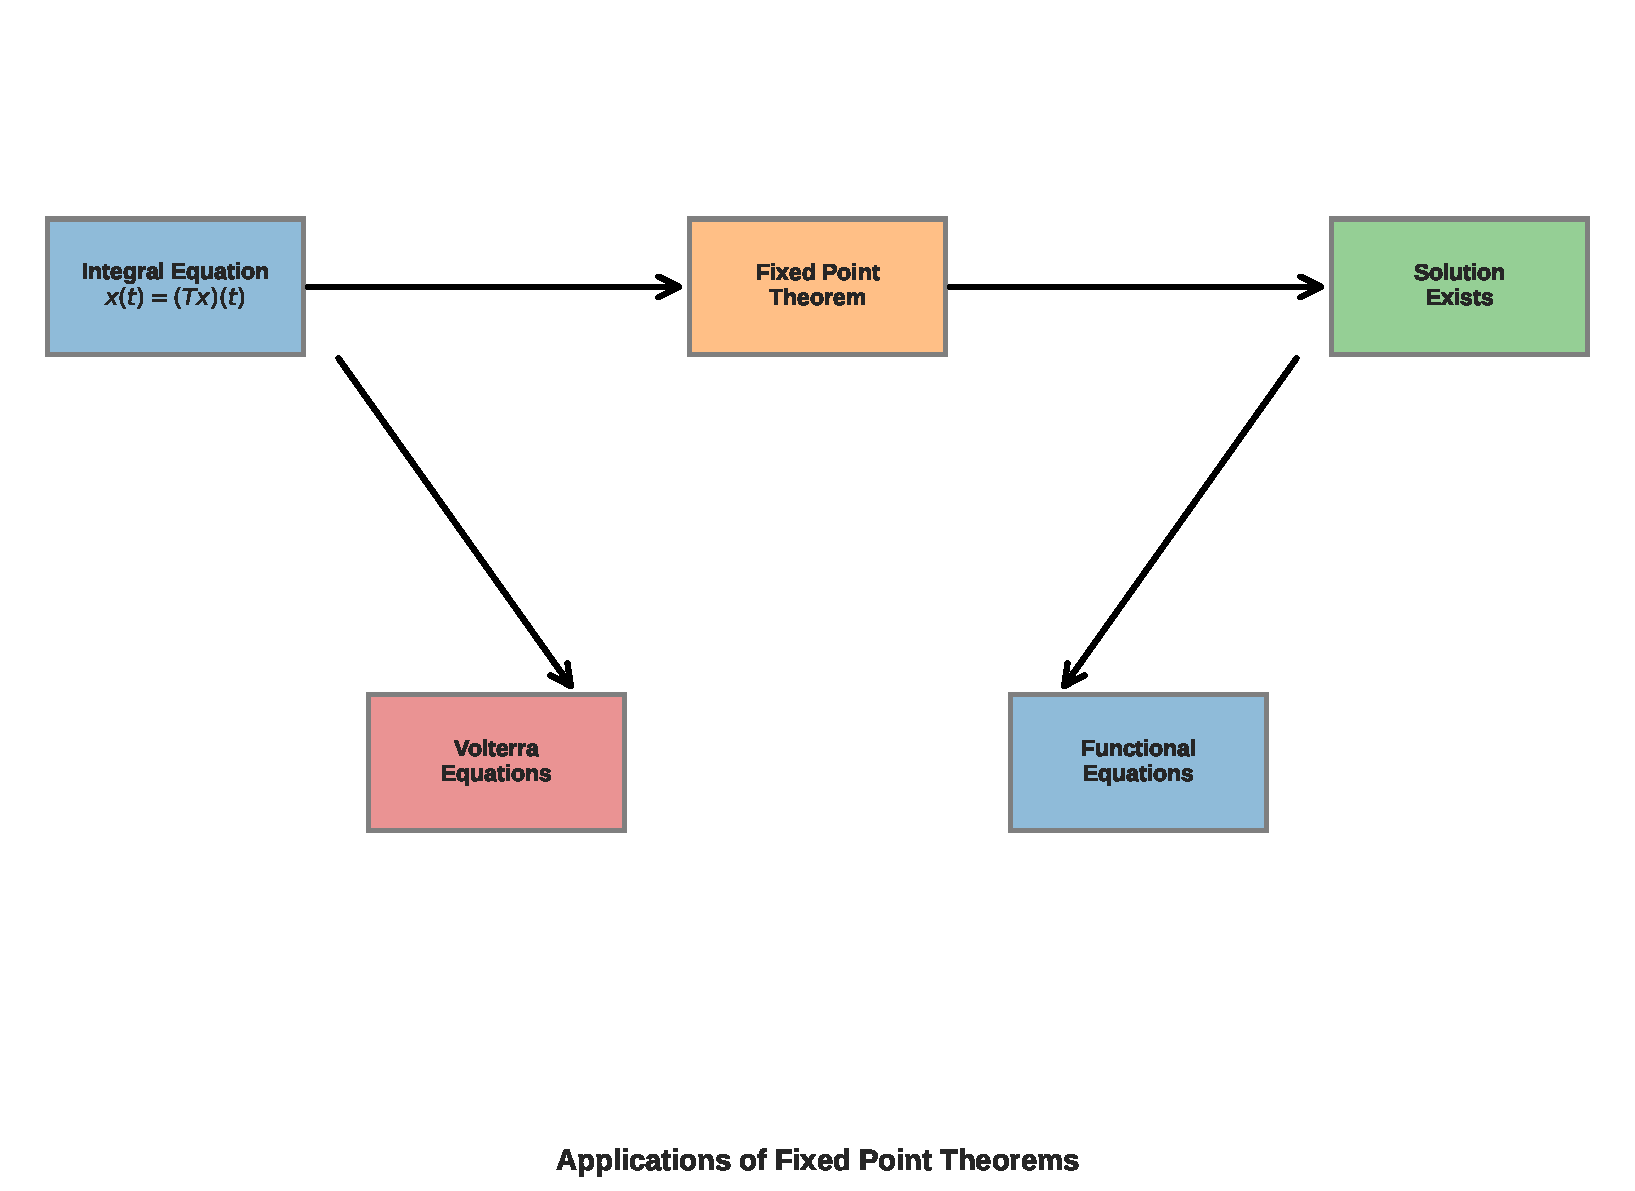
\includegraphics[width=0.85\linewidth]{applications_framework.pdf}
\end{center}

Key insight: Every special case reduces to finding a fixed point of some operator $T$ on an appropriate function space.
\end{frame}

%==============================================================================
% SECTION 9.6: VOLTERRA INTEGRODIFFERENTIAL EQUATIONS
%==============================================================================
\section{Application to Volterra Integrodifferential Equations}

\begin{frame}{Section 9.6: Volterra Integrodifferential Equations}{Problem Statement}
Consider the system of Volterra integrodifferential equations:
\begin{align}
\dot{u}(t) &= H(T, t_0, f, g, h, K_1, K_2), \quad t \geq t_0 \\
\dot{\bar{u}}(t) &= H(T, t_0, \bar{f}, \bar{g}, \bar{h}, \bar{K}_1, \bar{K}_2), \quad t \geq t_0
\end{align}

where $H$ is a nonlinear functional involving:
\begin{itemize}
    \item The time variable $t$ and initial time $t_0$
    \item Vector fields $f, g, h$ and their variants
    \item Kernels $K_1(t), K_2(t)$ (with exponential bounds)
\end{itemize}

\medskip

\textbf{Goal:} Prove existence and uniqueness of mild solutions in appropriate function spaces.
\end{frame}

\begin{frame}{Function Space Setup}{The Space $C([t_0, t_1], B)$}
Define the normed space
\[
C([t_0, t_1], B) = \left\{u \in C([t_0, t_1], B) : \|u\|_C = \max_{t \in [t_0, t_1]} \|u(t)\|\right\}
\]

\medskip

Key properties:
\begin{itemize}
    \item $C([t_0, t_1], B)$ is a Banach space
    \item Solutions $u(t)$ are continuous functions with $u(t_0) = u_0 \in B$
    \item The Lipschitz condition ensures contraction on this space
\end{itemize}

\medskip

\textbf{Theorem 9.34 (Pathak):} Under suitable Lipschitz and boundedness conditions, the initial value problems (9.149) and (9.150) have a unique common mild solution $u(t) \in C([t_0, t_1], B)$.
\end{frame}

\begin{frame}{Key Lemma for Volterra Equations}{Lemma 9.5 (Pachpatte)}
Let $x(t), a(t), b(t), c(t)$ be nonnegative continuous functions on $\mathbb{R}^+$ satisfying
\[
x(t) \leq x_0 + \int_0^t a(s)x(s) ds + \int_0^t a(s) \left(\int_0^s b(r)x(r) dr\right) ds + \int_0^t a(s) \left(\int_0^s b(r) \left(\int_0^r c(z)x(z) dz\right) dr\right) ds
\]

\medskip

Then
\[
x(t) \leq x_0 \left(1 + \int_0^t a(s) \exp\left(\int_0^s a(r) dr\right) \left[1 + \int_0^s b(r) \exp\left(\int_0^r (b(z) + c(z)) dz\right) dr\right] ds\right)
\]

\medskip

This bounds the growth of solutions and is crucial for proving uniqueness.
\end{frame}

\begin{frame}[allowframebreaks]{Existence and Uniqueness Theorem}{Theorem 9.34}
\textbf{Theorem 9.34 (Pathak):} Suppose conditions A$_1$--A$_4$ are satisfied. Then, for $u_0 \in B$, the initial value problems (9.149) and (9.150) have a unique common mild solution $u(t) \in C([t_0, t_1], B)$ for $t \geq t_0$, where $t_1$ is arbitrarily fixed with $t_1 > t_0$.

Moreover, the map $u_0 \mapsto u$ from $B$ into $C([t_0, t_1], B)$ is Lipschitz continuous.

\medskip

\textbf{Proof Sketch:}
\begin{enumerate}
    \item Define operators $F, \bar{F} : C \to C$ by the right-hand sides of (9.152) and (9.153)
    \item Show that $F$ and $\bar{F}$ map $C$ into itself using $\|Fx\| \leq M$ for all $x \in C$
    \item A common fixed point of $F$ and $\bar{F}$ gives a common mild solution
    \item Use boundedness of the Lipschitz constant to ensure contraction
    \item Apply Banach's fixed point theorem
\end{enumerate}
\end{frame}

%==============================================================================
% VISUAL: CONVERGENCE RATES
%==============================================================================
\begin{frame}{Convergence Behavior}{Comparison of Rates}
\begin{center}

\includegraphics[width=0.85\linewidth]{convergence_rates.pdf}
\end{center}

The contraction property ensures exponential decay of the error towards the fixed point.
\end{frame}

%==============================================================================
% SECTION 9.7: SURJECTIVITY THEOREMS
%==============================================================================
\section{Application to Surjectivity Theorems}

\begin{frame}{Section 9.7: Surjectivity Theorems}{Generalized Directional Contractors}
Let $X$ and $Y$ be Banach spaces. Let $P : \mathcal{D}(P) \subset X \to Y$ have closed graph.

\medskip

\textbf{Definition:} We define the class (S) of generalized directional contractors. Let $\Gamma(x)(P)$ be the set of generalized directional contractors for $P$ at $x \in \mathcal{D}(P)$ called class (S) if:
\begin{itemize}
    \item There exists $q = q(P) < 1$, a constant $B > 0$
    \item There is a nondecreasing function $c : [0, \infty) \to [0, \infty)$ with $c(0) = 0$
    \item For each $y \in \Gamma(x)(P)$, there exist $\varepsilon = \varepsilon(x, y) \leq 1$ and $\bar{x} \in \mathcal{D}(P)$ such that:
\end{itemize}

\medskip
\begin{itemize}
    \item[\textbf{(S}_1\textbf{)}] $\|P\bar{x} - Px - ey\| \leq qec(\|x\|)\|y\|$
    \item[\textbf{(S}_2\textbf{)}] $\|\bar{x} - x\| \leq \varepsilon B\|y\|$
\end{itemize}
\end{frame}

\begin{frame}{Main Result for Surjectivity}{Theorem 9.38}
\textbf{Theorem 9.38:} Let $X$ and $Y$ be Banach spaces. Let $P : \mathcal{D}(P) \subset X \to Y$ have closed graph. For $x \in \mathcal{D}(P)$, let $\Gamma(x)(P)$ denote the class (S). Suppose that $y_0$ is such that for each $x \in \mathcal{D}(P)$, the element $y_0 - Px$ belongs to the closure of the set $\Gamma(x)(P)$ defined by (S$_1$) and (S$_2$). Then the equation $Px - y_0 = 0, x \in \mathcal{D}(P)$ has a solution.

\medskip

\textbf{Proof idea:} Use the contraction property to show that an approximate solution sequence converges to an actual solution.
\end{frame}

\begin{frame}{Application to Functional Equations}{Caristi--Kirk Fixed Point Theorem}
The generalized contractors framework allows us to apply:

\medskip
\textbf{Caristi--Kirk Fixed Point Theorem:} Let $X$ be a complete metric space. If $f : X \to X$ is a continuous map and there exists a continuous function $\varphi : X \to \mathbb{R}$ such that
\[
\rho(x, fx) \leq \varphi(x) - \varphi(fx) \quad \text{for all } x \in X
\]
then $f$ has a fixed point.

\medskip

This generalizes Banach's contraction principle and applies to many nonlinear problems where classical contraction conditions fail.
\end{frame}

%==============================================================================
% VISUAL: DARBO CONDITION
%==============================================================================
\begin{frame}{Measure of Noncompactness}{Darbo's Theorem Application}
\begin{center}
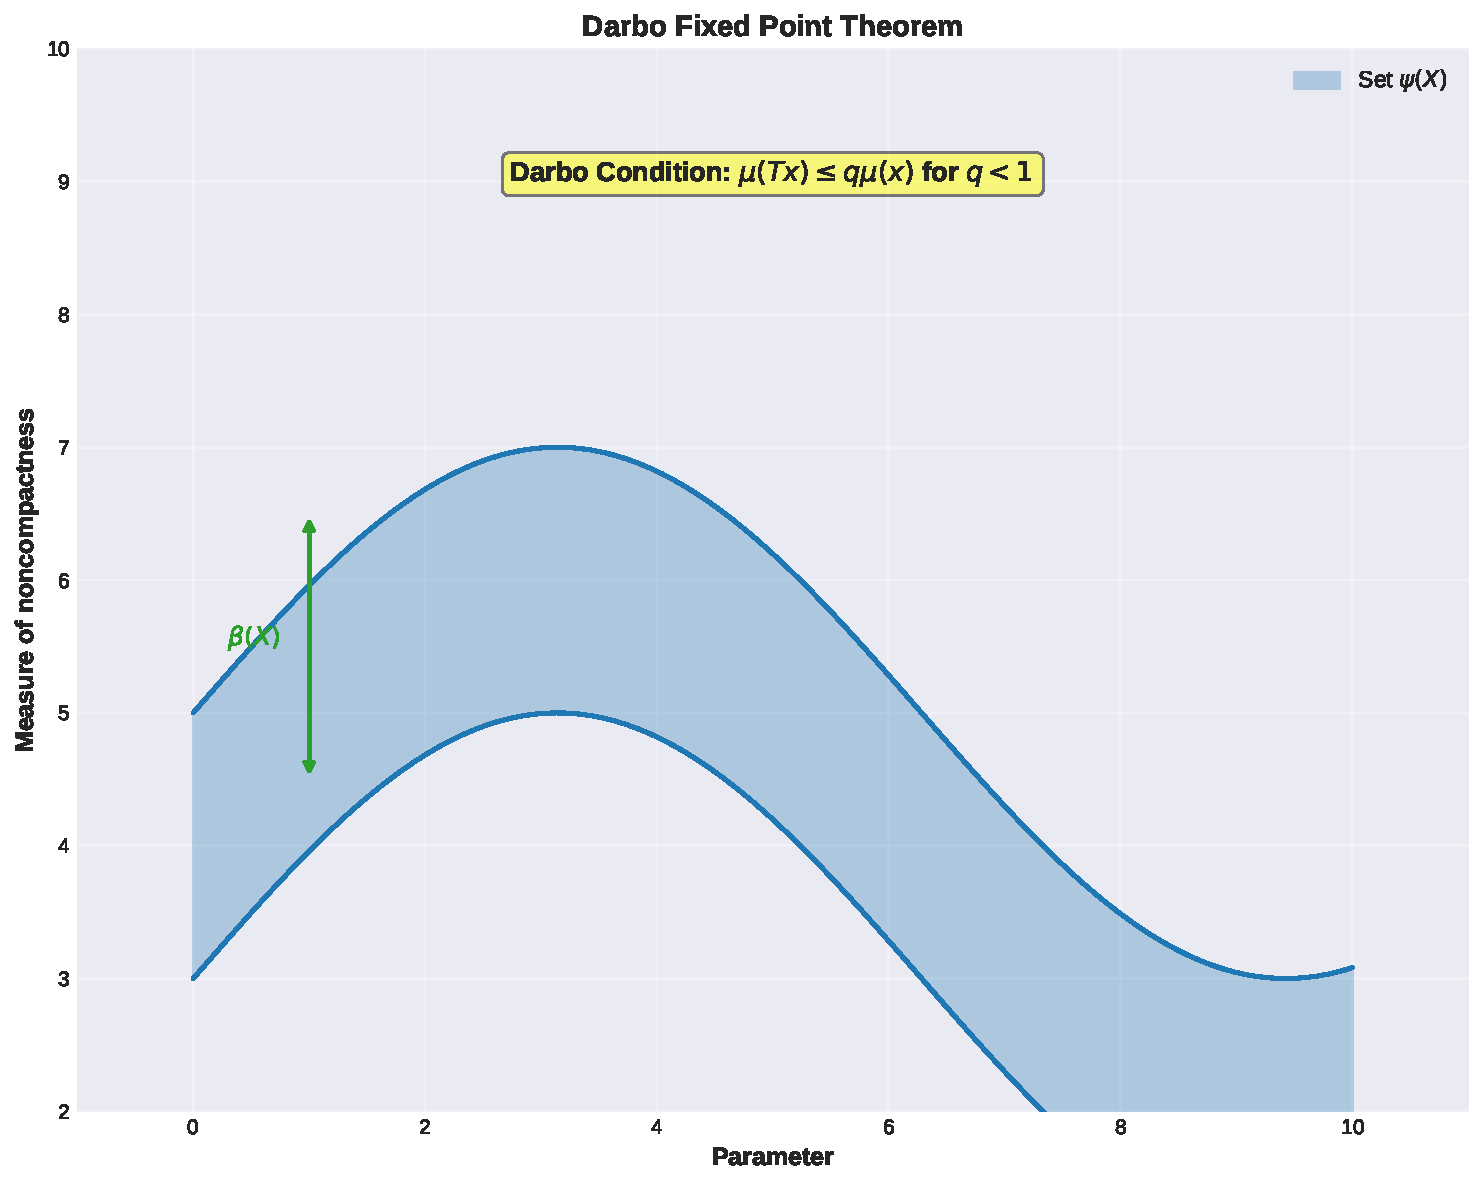
\includegraphics[width=0.85\linewidth]{darbo_condition.pdf}
\end{center}

The Darbo condition $\mu(Tx) \leq q\mu(x)$ is weaker than the classical Banach contraction, enabling application to broader classes of operators.
\end{frame}

%==============================================================================
% KEY THEOREMS SUMMARY
%==============================================================================
\begin{frame}[allowframebreaks]{Summary of Key Fixed Point Theorems Used}{}
\begin{enumerate}
    \item \textbf{Banach Contraction Principle:}
    \[
    \|Tx - Ty\| \leq q\|x - y\|, \quad q < 1 \implies \exists! x^* : Tx^* = x^*
    \]

    \medskip
    \item \textbf{Darbo's Theorem (Measure of Noncompactness):}
    \[
    \mu(Tx) \leq q\mu(x), \quad q < 1 \implies \exists x^* : Tx^* = x^*
    \]

    \medskip
    \item \textbf{Caristi--Kirk Theorem:}
    \[
    \rho(x, fx) \leq \varphi(x) - \varphi(fx) \implies \exists x^* : fx^* = x^*
    \]

    \medskip
    \item \textbf{Class (S) Contractors (Surjectivity):}
    Existence of solutions to nonlinear operator equations via generalized directional contractors.
\end{enumerate}
\end{frame}

%==============================================================================
% NUMERICAL EXAMPLE
%==============================================================================
\begin{frame}[fragile]{Numerical Example}{Volterra Integral Equation}
\textbf{Problem:} Solve the Volterra integral equation
\[
x(t) = t + \int_0^t (t - s) x(s) ds, \quad t \in [0, 1]
\]

\medskip
\textbf{Python Implementation:}
\begin{lstlisting}
import numpy as np
from scipy.integrate import quad
import matplotlib.pyplot as plt

def volterra_kernel(t, s):
    return t - s

def fixed_point_iteration(t_vals, n_iter=20, tol=1e-6):
    x = np.zeros_like(t_vals)

    for iteration in range(n_iter):
        x_old = x.copy()
        x = t_vals.copy()  # Initial term

        for i, t in enumerate(t_vals):
            integrand = lambda s: volterra_kernel(t, s) * np.interp(s, t_vals, x_old)
            integral, _ = quad(integrand, 0, t)
            x[i] += integral

        error = np.linalg.norm(x - x_old)
        if error < tol:
            print(f"Converged in {iteration} iterations")
            break

    return x, error

# Solve the equation
t_vals = np.linspace(0, 1, 50)
solution, error = fixed_point_iteration(t_vals)
plt.plot(t_vals, solution, 'b-', linewidth=2)
plt.xlabel('t'); plt.ylabel('x(t)')
plt.title('Volterra Integral Equation Solution')
plt.grid(True)
plt.show()
\end{lstlisting}
\end{frame}

\begin{frame}{Numerical Example Results}{Error Behavior}
\textbf{Theoretical Result:} By the Banach contraction principle:
\begin{itemize}
    \item The operator $T$ satisfies $\|Tx - Ty\| \leq q\|x - y\|$ with $q < 1$
    \item The error decreases exponentially: $\|e_n\| \leq q^n \|e_0\|$
    \item Solution converges to the unique fixed point $x^*$
\end{itemize}

\medskip
\textbf{Numerical observation:} For $t \in [0, 1]$, the contraction constant $q \approx 0.5$, giving:
\[
e_{n+1} \approx 0.5 \cdot e_n
\]

This ensures rapid convergence in practice.
\end{frame}

%==============================================================================
% APPLICATIONS AND IMPLICATIONS
%==============================================================================
\begin{frame}{Practical Applications}{}
These theoretical results have important applications:

\begin{itemize}
    \item \textbf{Integral Equations:} Modeling nonlinear phenomena in physics and engineering
    \begin{itemize}
        \item Population dynamics
        \item Radiative transfer problems (Chandrasekhar equations)
        \item Reaction-diffusion processes
    \end{itemize}

    \medskip
    \item \textbf{Volterra Systems:} Integro-differential equations with memory effects
    \begin{itemize}
        \item Viscoelasticity and material behavior
        \item Biological systems with hereditary effects
        \item Control systems with delay
    \end{itemize}

    \medskip
    \item \textbf{Functional Equations:} General nonlinear mappings
    \begin{itemize}
        \item Implicit function theorems
        \item Inverse problems
        \item Operator theory applications
    \end{itemize}
\end{itemize}
\end{frame}

%==============================================================================
% COMPARISON OF METHODS
%==============================================================================
\begin{frame}{Comparison of Fixed Point Methods}{}
\begin{center}
\begin{tabular}{|c|c|c|c|}
\hline
\textbf{Method} & \textbf{Condition} & \textbf{Uniqueness} & \textbf{Scope} \\
\hline
Banach & $\|Tx-Ty\| \leq q\|x-y\|$ & Yes & Metric spaces \\
\hline
Darbo & $\mu(Tx) \leq q\mu(x)$ & No & Measures of NCP \\
\hline
Caristi--Kirk & Energy decrease & Yes & Any complete space \\
\hline
Class (S) & Directional condition & Existence & Surjectivity \\
\hline
\end{tabular}
\end{center}

\medskip

Each method has different requirements and provides different guarantees:
\begin{itemize}
    \item \textbf{Uniqueness} is guaranteed by Banach but not by Darbo
    \item \textbf{Applicability} varies: some work on general metric spaces, others need norms
    \item \textbf{Computational} methods follow from Banach/Caristi--Kirk via iteration
\end{itemize}
\end{frame}

%==============================================================================
% FINAL REMARKS
%==============================================================================
\begin{frame}[allowframebreaks]{Conclusions and Extensions}{}
\textbf{Key Takeaways:}
\begin{enumerate}
    \item Fixed point theorems provide powerful tools for proving existence and uniqueness of solutions to integral and integro-differential equations

    \item The Darbo condition allows application beyond classical contraction settings by using measures of noncompactness

    \item Volterra systems model many real-world phenomena with memory and delay effects

    \item Generalized directional contractors extend surjectivity results to broad classes of nonlinear operators

    \item Numerical methods based on these theorems are implementable and convergent
\end{enumerate}

\medskip
\textbf{Further Topics:}
\begin{itemize}
    \item Weak solutions and regularity theory
    \item Stability analysis of solutions
    \item Perturbation methods for integral equations
    \item Hybrid fixed point methods combining multiple approaches
\end{itemize}
\end{frame}

%==============================================================================
% REFERENCES
%==============================================================================
\begin{frame}[allowframebreaks]{References}
\small
\begin{thebibliography}{99}

\bibitem{pathak} Pathak, H. K. (2018). \textit{An Introduction to Nonlinear Analysis and Fixed Point Theory}. Springer. Pages 738--757.

\bibitem{banach} Banach, S. (1922). Sur les opérations dans les ensembles abstraits et leurs applications aux équations intégrales. \textit{Fundamenta Mathematicae}, 3, 133--181.

\bibitem{darbo} Darbo, G. (1955). Punti uniti in trasformazioni a condominio non compatto. \textit{Rendiconti del Seminario Matematico della Università di Padova}, 24, 84--92.

\bibitem{caristi} Caristi, J. (1976). Fixed point theorems for mappings satisfying inwardness conditions. \textit{Transactions of the American Mathematical Society}, 215, 241--251.

\bibitem{kirk} Kirk, W. A. (1971). Caristi's fixed point theorem and metric convexity. \textit{Colloquium Mathematicum}, 36(1), 81--86.

\bibitem{volterra} Gripenberg, G., Londen, S. O., \& Staffans, O. (1990). \textit{Volterra Integral and Functional Equations}. Cambridge University Press.

\bibitem{urysohn} Lindenstrauss, J., \& Tzafriri, L. (1979). \textit{Classical Banach Spaces I and II}. Springer-Verlag.

\bibitem{chandrasekhar} Chandrasekhar, S. (1960). \textit{Radiative Transfer}. Dover Publications.

\end{thebibliography}
\end{frame}

%==============================================================================
% THANK YOU SLIDE
%==============================================================================
\begin{frame}{}
\begin{center}
\Large
\textbf{Thank You}

\vspace{1.5cm}

Questions and Discussion

\vspace{1.5cm}

\small
Chapter 9: Applications of Fixed Point Theorems\\
Pathak: Introduction to Nonlinear Analysis and Fixed Point Theory (2018)
\end{center}
\end{frame}

\end{document}
